\chapter{Bayesian Inference as a Cognitive Account}
\label{sec:p19-bayesian-cognitive-inference}

Bayes's identity does not, by itself, specify a theory of human learning.
A cognitive account must identify the hypotheses a learner considers,
the data available, the prior constraints, the observation model and the
response being explained. Griffiths, Tenenbaum and Kemp's Oxford chapter~3
develops this approach for induction in categories, causal relationships
and language. Its central contribution is a common framework capable of
working with different structured representations, not one universal
hypothesis space or a claim that every person explicitly computes a posterior
\cite[pp.~22--35]{GriffithsTenenbaumKemp2012BayesianInference}.

The account connects prior-sensitive everyday predictions, structured
hypothesis spaces and hierarchical learning. Its review illustrations
are distinguished from an original human function-learning experiment
and a bounded formal analysis of iterated learning. Normative identities,
assumptions about environments, behavioral correspondence, algorithms
and neural implementation receive different evidential standings.

\section{Hypotheses, data, priors and likelihoods}
\label{sec:p19-bci-model}

\begin{hbdefinition}{def:p19-bci-model}{A finite cognitive inference model}
Let \(H\) be a finite nonempty hypothesis space and \(\mathcal D\) a
finite nonempty data alphabet. A hypothesis \(h\in H\) can be a total
duration, a category extension, a graph, a grammar or another specified
structure. Let \(\pi(h)=P(h)\) be nonnegative prior masses summing to
one. A likelihood \(L(d\mid h)=P(d\mid h)\) is a data distribution
for each hypothesis: nonnegative and summing to one over \(d\in\mathcal D\).
After observation \(d\), it is evaluated as a function of \(h\), not
as a probability distribution over hypotheses.

The prior predictive mass is
\[
 m(d)=\sum_{h\in H}\pi(h)L(d\mid h).
\]
For \(m(d)>0\), posterior masses are
\[
 q_d(h)=P(h\mid d)=\frac{L(d\mid h)\pi(h)}{m(d)}.
\]
This is the finite reading of the chapter's equation~1. The sum version
does not silently cover an arbitrary continuous or infinite space;
\cref{thm:p15-bayes-posterior-kernel} supplies a proper-prior dominated
extension under its measurability and regular-observation conditions.
\index{Bayesian inference!cognitive models}
\index{rational analysis!cognition}
\end{hbdefinition}

\begin{hbtheorem}{thm:p19-bci-bayes}{proved=annex:p19.bci.bayes}{Finite updating and a prediction--diagnosis contrast}
The preceding prior and likelihood define a joint law on \(H\times\mathcal D\).
For \(m(d)>0\), \(q_d\) is exactly its conditional hypothesis law.
If a finite future response alphabet has nonnegative conditional masses
\(K(y\mid h,d)\) summing to one over \(y\) for each \(h,d\),
then \(\sum_hq_d(h)K(y\mid h,d)\) is a normalized predictive law.
Prior-zero hypotheses retain zero posterior mass; \(m(d)=0\) does not
define a posterior by division.

Under five independent fair coin tosses, the exact ordered strings HHTHT
and HHHHH each have probability \(1/32\). Under a separate deterministic
all-heads hypothesis, HHHHH has probability one and HHTHT zero. Thus equal
predictive probabilities under the fair model do not imply equal diagnostic
support when another specified model is compared.
\end{hbtheorem}

The coin contrast makes the source's discussion of subjective randomness
precise. A person may be evaluating how much a string supports randomness
against a structured alternative, rather than which exact string is most
likely under an already-stipulated fair process. These are different questions.
Finding a plausible diagnostic interpretation does not establish that a
participant used it, or make the predictive answer to the original question
correct. Distinctive task manipulations are needed to test that interpretation
\cite[pp.~26--27]{GriffithsTenenbaumKemp2012BayesianInference}.

The chapter's opening predictions concern a man already aged~60 and a
movie that has earned \$40 million so far. Hypotheses are total lifespan or
total gross; observed age or current receipts are data. A prior describes
the relevant total-quantity distribution, while the likelihood describes
how an observation at that partial amount is encountered given the total.
Totals below the observed amount are excluded by that interpretation, but
the remaining weighting still depends on the encounter/observation process.
A prior alone is not an observation model. These are source illustrations,
not current life-expectancy advice or financial forecasts
\cite[pp.~23--24]{GriffithsTenenbaumKemp2012BayesianInference}.

\section{A computational solution is not an implementation}
\label{sec:p19-bci-levels}

Marr's computational level asks which problem is solved and what an ideal
solution looks like; the algorithmic level concerns representations and
processes; the implementation level concerns realization in hardware.
The chapter's principal Bayesian analyses begin at the computational level.
Their large hypothesis spaces and probability distributions characterize
the inference problem, not necessarily an explicit list stored by a person.
Behavioral similarity to a posterior-based prediction does not by itself
identify its algorithm or neural realization
\cite[pp.~23--25]{GriffithsTenenbaumKemp2012BayesianInference}.

The authors contrast this function-first approach with cognitive architectures
and connectionist models emphasizing mechanistic components. A production
rule or neural-network unit is often proposed as a process component,
whereas a computational prior may initially represent a constraint on
knowledge. The approaches need not exclude one another. Rational process
models propose psychologically interpretable approximations to Bayesian
inference, including Monte Carlo sampling; proposed spiking-network
implementations operate at another explanatory level. Neither reference
to a sampling algorithm nor its effectiveness in a computer establishes
that the brain implements that particular sampler.

The source uses rationality differently in reverse engineering than in
standard error assessment. In the latter, a specified normative model is
compared with behavior. In reverse engineering, assuming that behavior
serves a reasonable function guides discovery of the problem, objective
and approximations. Rationality is then a methodological starting point,
not a finding already established about all responses. Bounded, approximate
or local optimization may be relevant; global optimality is not guaranteed.
The chapter's comparison with the machine-learning capabilities of its
period is a dated motivation, not a current performance claim.

\section{The heuristics-and-biases comparison and its objections}
\label{sec:p19-bci-rivals}

The source distinguishes explicit judgments about statistics, money and
policy from many implicit judgments using ordinary observations in
categorization, causal learning or language. Success in one setting does
not refute failures in another. Nor does this contrast prove that all
implicit cognition is optimal or every explicit probability judgment is
defective. The chapter recognizes overlap between the traditions and
offers two kinds of reconciliation
\cite[pp.~25--27]{GriffithsTenenbaumKemp2012BayesianInference}.

First, a response can be sensible under a different task construal. The
source cites information-gain interpretations of Wason's selection task,
pragmatic information conveyed by apparently equivalent frames, diagnostic
randomness judgments and coincidence detection as evidence for a hidden
structured cause. Each reinterpretation changes the stated inference
problem. It needs quantitative tests of predictions against compelling
alternatives, not an after-the-fact story that can explain every answer.
The authors explicitly acknowledge this danger.

A heuristics-and-biases explanation may instead call the reinterpretation
task substitution. A substituted problem can itself have a rational
solution while producing a harmful error on the problem the situation
actually requires. Computational justification of a shortcut is not proof
that using it here served the person's aims. This preserves the disagreement
about what participants interpreted and which interpretation the normative
assessment should use.

Second, some responses resist a plausible Bayesian reinterpretation.
The source treats them as opportunities to identify approximate mechanisms,
not a reason to declare all departures optimal. It also compares adaptive
simple heuristics with flexible statistical models. A heuristic tuned to
environmental structure may generalize better than an underconstrained
maximum-likelihood model. The authors invoke the bias--variance tradeoff
and suggest comparing models with analogous environmental assumptions.
That is a conditional explanation of the comparison; it does not prove
every Bayesian method beats every heuristic or that all approximation
errors are harmless.

\Cref{sec:p19-rationality-4-5} develops the distinct Bayesian verbal-reasoning
presentation, including conditional interpretation and information selection.
Its formal coherence constraints do not by themselves validate the present
chapter's cognitive hypotheses. Conversely, a probability model for
induction is not a counterexample to classical deduction under fixed
premises and semantics. A fair comparison holds the task, interpreted
information and criterion constant before comparing predictions.

\section{Everyday prediction: what Figure 3.1 actually reports}
\label{sec:p19-bci-everyday}

The source adapts Griffiths and Tenenbaum's 2006 prediction illustration.
Its upper panels show empirical total-quantity distributions; lower panels
show median participant predictions against Bayesian curves using empirical
and fitted priors, plus a common uninformative-prior comparison. The five
displayed domains are life spans, movie runtimes, movie grosses, poem
lengths and representatives' terms. The first two displayed distributions
are peaked, approximately Gaussian; movie grosses and poems are the
heavy-tailed, approximately power-law examples; terms supply the
approximately Erlang example. The domain order matters to the model
comparison rather than being interchangeable decoration.

The reported correspondence is an aggregate judgment pattern. The chapter
does not supply participant recruitment, sample size, trial assignments,
exact fitted parameters, numerical fit statistics or the numerical endpoints
of the displayed uncertainty bars. No such fields are reconstructed here
from the image. A median match does not show that every participant has
the fitted prior, or uniquely identify an explicit conditionalization
process. An alternative response model, aggregation across heterogeneous
strategies or different assumptions about encountering observations can
matter \cite[pp.~23--24, fig.~3.1]{GriffithsTenenbaumKemp2012BayesianInference}.

The appropriate conclusion at this scope is that the authors use
domain-sensitive prediction patterns to motivate prior-sensitive cognitive
models. It is not a population estimate of universal Bayesian competence.
The empirical curves are not recreated with invented raw points or fitted
parameters. The original journal body's participant and model-fit record
remains distinct from this source-reviewed illustration.

\section{Symbols and statistics: source-specific hypothesis spaces}
\label{sec:p19-bci-representations}

Bayesian inference need not restrict hypotheses to arrays of numerical
weights. The chapter explicitly includes graphs, grammars, predicate logic,
relational schemas and functional programs. Statistics can then learn
structured symbolic hypotheses. This is not a claim that every symbolic
architecture is Bayesian or that every connectionist model lacks structure.
It challenges the simple opposition between symbolic representation and
statistical learning \cite[pp.~27--28]{GriffithsTenenbaumKemp2012BayesianInference}.

The source maps categorization to labeled category examples and hypotheses
about groupings; causal learning to observed variables and hypotheses about
causal structures; and language learning to utterances and hypotheses about
grammars or probabilistic utterance schemes. For biological properties,
tree proximity may encode expectations of shared features. Its protein-X
example considers extending information about cows and rhinos to horses or
squirrels. The chapter also stresses that trees are not universal:
geographic properties can require spaces/grids, value or ability comparisons
orders, and transmitted properties directed networks.

Its hypothetical medical map distinguishes a cold, coughing, fever, lung
disease and chest pain to illustrate graph structure. Such a toy graph's
arrows specify proposed model dependencies, not clinical evidence that
those causes exhaust the symptoms. A graph alone also does not specify
all conditional probabilities, confounder assumptions or intervention
semantics. The higher-level disease/symptom schema constrains which
directions of edges a learner expects, rather than supplying a medical
diagnosis. Distinguishing an edge's existence from its strength is another
source contribution; posterior inference about one does not automatically
answer the other.

For the structure-learning hierarchy, \(F\) is a form grammar, \(G\)
a graph produced by it and \(D\) an observed data matrix, rather than
the data alphabet \(\mathcal D\) in the finite benchmark. The factored
generative model \(P(F)P(G\mid F)P(D\mid G,F)\) makes the hierarchy
explicit. Choosing its factors and a search procedure remains a
model-construction task.

\begin{figure}[htbp]
\centering
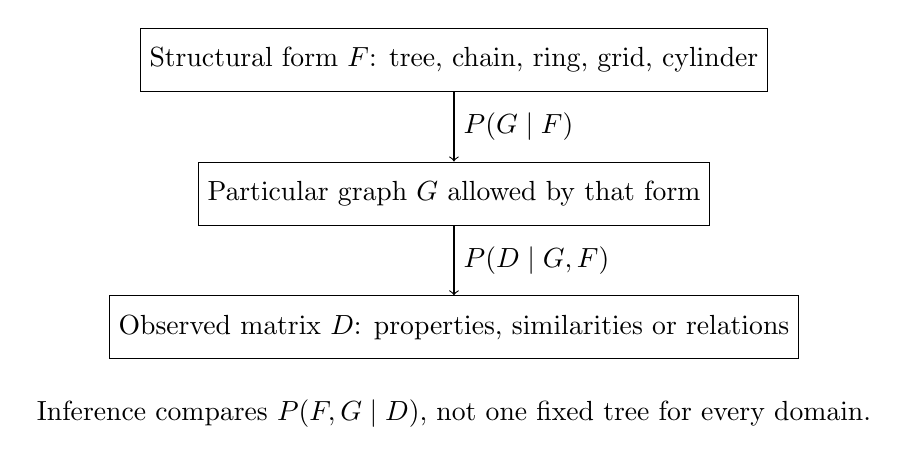
\begin{tikzpicture}[x=1cm,y=1cm]
\node[draw,minimum width=6.2cm,minimum height=.8cm,align=center] (form) at (0,4) {Structural form \(F\): tree, chain, ring, grid, cylinder};
\node[draw,minimum width=6.2cm,minimum height=.8cm,align=center] (graph) at (0,2.3) {Particular graph \(G\) allowed by that form};
\node[draw,minimum width=6.2cm,minimum height=.8cm,align=center] (data) at (0,.6) {Observed matrix \(D\): properties, similarities or relations};
\draw[->] (form.south)--node[right]{\(P(G\mid F)\)}(graph.north);
\draw[->] (graph.south)--node[right]{\(P(D\mid G,F)\)}(data.north);
\node[align=center] at (0,-.5) {Inference compares \(P(F,G\mid D)\), not one fixed tree for every domain.};
\end{tikzpicture}
\caption{Native explanatory diagram of the hierarchy in source Figure~3.3.
It preserves form, structure and data as different levels without pretending
to reproduce the source's fitted animal, voting, color, face or city data.}
\label{fig:p19-bci-hierarchy}
\end{figure}

Source Figure~3.3 says that an algorithm \emph{attempts} to find
a high-posterior form/graph pair; it does not prove that every search finds
the global optimum.

The examples retain different data types: animal features favor a tree;
judges' voting patterns a linear ordering; color similarities a ring;
the source's two manipulated face dimensions a grid; and geographic
proximities a cylindrical organization analogous to latitude/longitude.
These are reviewed model demonstrations, not a controlled comparison
showing that human participants recovered all five representations or
that the selected form is uniquely true of every such domain.

\begin{hbtheorem}{thm:p19-bci-tree-count}{proved=annex:p19.bci.tree-count}{The tree restriction and its counting convention}
A set of \(n\geq2\) distinct objects has \(2^n\) subsets. A fixed
rooted full binary tree with those objects as its leaves has \(n-1\)
internal nodes, hence \(n-1\) distinct nonsingleton descendant-leaf clades.
Allowing just those clades supplies the restricted \(n-1\) candidate
concepts used in the source's comparison. Including singleton leaves gives
\(2n-1\) clades; literally counting edges gives \(2n-2\). Thus the
source's shorthand about branches requires an explicit candidate convention.
\end{hbtheorem}

The reduction illustrates an inductive constraint; it does not establish
that the fixed tree is the correct one, where it comes from, or that
every actual category is a clade. A restricted space that excludes the
data-generating structure cannot recover it by updating alone.

\section{Identifying priors and iterated learning}
\label{sec:p19-bci-iterated}

The chapter gives three routes to studying inductive constraints: comparing
prior-dependent predictions with task data; asking which priors would make
observed learning possible from the available information, including
linguistic corpora; and designing procedures intended to reveal priors.
Each depends on likelihood and response assumptions as well as the prior.
An explanation by one fitted prior is not proof that no alternative model
can explain the observations.

Iterated learning supplies the third route. One learner receives data,
selects a hypothesis and produces data for the next learner. The 2007
formal paper distinguishes sampling from a posterior from selecting a
maximum-posterior hypothesis. Merely using Bayes's identity does not fix
that selection rule. Stationarity and convergence are also different
claims; convergence requires mixing conditions
\cite[pp.~29--30]{GriffithsTenenbaumKemp2012BayesianInference}
\cite[pp.~444--447,453--457,459--460]{GriffithsKalish2007IteratedAgents}.

\begin{hbtheorem}{thm:p19-bci-iterated}{proved=annex:p19.bci.iterated}{A complete finite posterior-sampling guarantee}
Assume the finite model in \cref{def:p19-bci-model}, with
\(\pi(h)>0\) and \(L(d\mid h)>0\) for every \(h,d\).
All learners have the same prior/likelihood. Given hypothesis \(j\),
produce \(d\) from \(L(d\mid j)\), then sample the next hypothesis
\(i\) from \(q_d\). Define the column-stochastic transition matrix
\[
 Q_{ij}=\sum_{d\in\mathcal D}q_d(i)L(d\mid j).
\]
This orientation matches the original's destination-first indices.
The prior is stationary, \(Q\pi=\pi\), and every initial hypothesis
distribution converges to it. The generated-data distribution converges
to \(m\). The annex gives an explicit geometric contraction bound.
Replacing posterior sampling by MAP selection need not preserve the prior;
removing mixing conditions can preserve the initial hypothesis indefinitely.
\end{hbtheorem}

\subsection{The original function-learning experiment}

Kalish, Griffiths and Lewandowsky's 2007 experiment supplies an actual
human task record rather than assuming that participants are the agents
in the theorem. It recruited 288 undergraduate psychology students at the
University of Louisiana at Lafayette for partial course credit: 72 per
initial-function condition, organized into eight families of nine learners
per condition, hence 32 transmission families. Ages, gender composition,
probability sampling, a prospective power calculation and a random
condition-assignment procedure are not reported
\cite[pp.~290--291]{KalishGriffithsLewandowsky2007Iterated}.

Participants worked individually in sound-attenuated booths. An input
\(x\) was displayed as a blue bar, and an unmarked mouse-controlled
slider set a red response bar representing \(y\). Values ran from 1
to 100. Initial targets were positive linear \(y=x\), negative linear
\(y=101-x\), a nonlinear U-shaped function, or random one-to-one
pairings. Fifty input values were drawn for training; values were rounded
to integers. The 50-item test used 25 training inputs and 25 previously
unused inputs. Each learner's test responses became the next learner's
training targets, without personal contact or disclosure of that transmission
role.

Training trials gave feedback. Accuracy within five units of target
yielded a one-second study interval; an error produced a tone, required
matching the feedback bar and yielded two seconds of study, followed
by a two-second blank interval. Test trials had no feedback. Thus initial
function conditions and the gradually changed target sets were defined,
but learners' errors also affected feedback exposure. These conditions
must not be replaced by a claim of unrestricted natural cultural transmission.

Twenty-eight of the 32 families reached a positive linear response
function in a few generations. Three ended with a negative linear function,
and one had not converged by the ninth generation. Eleven families
transmitted a negative linear function at least once. The quantitative
summary uses each learner's correlation with \(y=x\), summarized by
medians across families because negative-function outliers affect means.
No table of coefficient values, confidence intervals for the human
correlations or inferential test is supplied. The article's 1,000-chain
simulation intervals concern Bayesian agents, not 1,000 human participants
\cite[pp.~291--292, fig.~3]{KalishGriffithsLewandowsky2007Iterated}.

Source Figure~3.2 displays selected positive-convergence trajectories.
The primary paper's text calls its examples representative, whereas its
figure caption calls the rows randomly drawn; no selection protocol resolves
that difference. In either case, the displayed rows are not all 32 families.
The original also includes the negative outcome and explicitly states
that substantially more data would be needed to confirm stationarity and
map the distribution. These qualifications prevent upgrading a tendency
in the study into universal convergence or proof that human learners
sampled their mathematical posteriors.

The prior may encode acquired or domain-general constraints; a transmission
pattern does not show that a bias is innate or specific to language.
The paper's two notes preserve those limitations. Function learning is
the measured task. Generalization to language, legends or norms remains
an interpretation requiring separate evidence, not an additional outcome
measured in these students.

\section{Hierarchies, causal schemas and abstraction}
\label{sec:p19-bci-hierarchies}

The source's hierarchical Bayesian account puts priors on structures and
on the higher-level constraints determining those structures. Learning
can then occur at several levels, with higher-level knowledge constraining
lower-level inferences while evidence below informs the higher levels.
This does not eliminate assumptions: the possible hyperstructures,
hyperpriors, generative factors and search procedures still must be supplied.

Figure~3.4 is a computational illustration with sixteen hypothetical
condition variables: six disease nodes and ten symptom nodes. A two-level
network/data model with a weak structural prior is contrasted with a
three-level class-schema/network/data model favoring class~\(C_1\)
to class~\(C_2\) links. The caption reports little specific-network
learning at 20 records and spurious links at 80 in the two-level model;
the three-level model learns the class-level organization at 20 and
nearly recovers the illustrated network at 80. A 1,000-record comparison
is mentioned but not shown. Those record counts index the model's data,
not a clinical trial or a demonstrated human sample size requirement
\cite[pp.~30--32, figs.~3.3--4]{GriffithsTenenbaumKemp2012BayesianInference}.

The chapter uses these results to motivate learning a framework before
all its specific relations. The blessing-of-abstraction explanation is
that a higher-level constraint pools evidence from many lower-level
variables. It is a property of particular model structures, not a theorem
that every abstraction is learned faster or that adding layers always
improves predictive accuracy. The source contrasts this approach with
selected nativist and bottom-up associationist accounts. Its stronger
suggestion that only HBMs suit early learned abstraction is an argumentative
assessment, not an independently established exclusion of every rival
developmental mechanism.

The historical Linnaeus tree and Mendeleev periodic-structure examples
illustrate discovering a form rather than fitting parameters within a
single predetermined form. They are not reconstructions of those
discoveries by a human subject model. The available form grammar limits
what a computational learner can discover; calling the process structure
discovery does not make an unprovided representation available.

\section{Connections, open problems and consultation}
\label{sec:p19-bci-use}

The source relates exemplar/prototype categorization to density estimation,
rational categorization to nonparametric Bayesian methods, causal induction
to graph structure/strength distinctions, and learning/perception to
conditioning, multisensory integration and perceptual organization.
These correspondences create hypotheses and mathematical tools; they
do not establish an identical cognitive mechanism across all those tasks.
Its later examples include single-sample decision tradeoffs, Church-style
probabilistic programs, relational and feature-discovery models. This
chapter does not give each named algorithm's complete correctness or
optimality proof, and the single-sample advantage is conditional on a
particular gain/time tradeoff rather than a universal prescription
\cite[pp.~31--33]{GriffithsTenenbaumKemp2012BayesianInference}.

The conclusion seeks to move beyond empiricism/nativism, domain-general/
domain-specific and symbol/statistics dichotomies by asking how learned
representations and constraints cooperate. It identifies developing
mechanistic accounts and explaining rapidly learned structured knowledge
as open research directions. A common Bayesian language does not make
the model-building or empirical-validation problems disappear.

\begin{hbmethod}{def:p19-bci-assessment}{Assess a Bayesian cognitive account}
State the inference question, the hypothesis representation, data and
observation mechanism. Give the prior, likelihood and posterior-to-response
rule; check evidence support rather than dividing by zero. Preserve the
source's representation variant instead of treating all models as one formula.

Identify the explanatory level and claim: conditional mathematical identity,
normative comparison, descriptive fit, approximate algorithm or implementation.
Show which evidence could distinguish competing models with similar outputs.
Do not use a computational fit as its own mechanism test.

Map every human outcome to its population, task, instructions, design,
measure, uncertainty, selection and dependence structure. Separate human
learners from simulations, medians from individuals and data records from
participants. State unavailable fields as unavailable.

For a rival comparison, hold the interpreted question and environmental
assumptions explicit. A changed task construal can explain a response
without answering the original task correctly. A heuristic comparison
needs a comparable treatment of structural constraints and flexibility.

Conclude at the justified scope: success on a particular prior-sensitive
task, a conditional convergence theorem or a model demonstration is not
universal Bayesian competence, guaranteed global search or current clinical
knowledge. Retain any source-level unresolved mechanism or empirical gap.
\end{hbmethod}

Successful cases are finite updating on supported evidence, the coin
prediction/diagnosis distinction, a declared tree restriction and the
posterior-sampling guarantee with its mixing assumptions. Failure cases
are selecting an omitted hypothesis, confusing likelihood with posterior,
inferring neural machinery from fit, assuming MAP transmission preserves
the prior, or reading selected positive trajectories as every family's
outcome. \Cref{sec:p15-bayesian-updating-prediction,sec:p15-bayesian-model-comparison}
supplies the general mathematical interfaces; \cref{def:p19-evidence-record}
supplies the empirical discipline. Neither substitutes for the source's
particular cognitive model, experiment or admitted boundary.
